\documentclass[lettersize,journal]{IEEEtran}
\usepackage{amsmath,amsfonts}
\usepackage{algorithmic}
\usepackage{algorithm}
\usepackage{array}
\usepackage[caption=false,font=normalsize,labelfont=sf,textfont=sf]{subfig}
\usepackage{textcomp}
\usepackage{stfloats}
\usepackage{url}
\usepackage{verbatim}
\usepackage{graphicx}
\usepackage{cite}
\hyphenation{op-tical net-works semi-conduc-tor IEEE-Xplore}
% updated with editorial comments 8/9/2021



% ====== Pakete (bei Bedarf anpassen) ======
\usepackage[utf8]{inputenc}    % Umlaute
\usepackage[T1]{fontenc}
\usepackage{graphicx}
\usepackage{amsmath,amssymb}
\usepackage{cite}
\usepackage{url}
\usepackage{array}
\usepackage{algorithmic} % falls ihr wirklich Algorithmen braucht

% ====== Dokumentbeginn ======
\begin{document}
\title{Künstliche Intelligenz in Wissenschaft und Medizin: 
	Potenziale, Verlässlichkeit und Evaluierungsstandards}

\author{Faik~Hadutoglu, Nico~Lang, Nikolaj~Schmidt%
	\thanks{Studiengang Fahrzeugelektronik (TFE23-2), DHBW Ravensburg.}%
}


\markboth{Seminararbeit -- Künstliche Intelligenz in Wissenschaft und Medizin}%
{Lang \MakeLowercase{\textit{et al.}}: Künstliche Intelligenz in Wissenschaft und Medizin}

	
	\maketitle
	
	% ====== Abstract & Keywords ======
\begin{abstract}
	Künstliche Intelligenz spielt eine wachsende Rolle in der medizinischen Diagnostik und biomedizinischen Forschung. Die vorliegende Arbeit analysiert Methoden zur systematischen Bewertung KI-gestützter Diagnoseverfahren und untersucht erforderliche Standards zur Sicherstellung von Reproduzierbarkeit, Fairness und Transparenz. Anhand einer Literaturauswertung aktueller Studien sowie regulatorischer Vorgaben (WHO, FDA, EU-MDR) werden Potenziale, Risiken und Bewertungsverfahren medizinischer KI-Systeme erörtert. Es zeigt sich, dass KI bei bestimmten diagnostischen Fragestellungen gute Ergebnisse liefert, gleichzeitig aber Probleme wie systematische Verzerrungen, eingeschränkte Reproduzierbarkeit und fehlende Nachvollziehbarkeit der Entscheidungsprozesse auftreten. Eine Zusammenarbeit von Mensch und KI mit definierter Aufgabenteilung und fortlaufender Überwachung erscheint als vielversprechendster Weg für einen sicheren klinischen Einsatz.
\end{abstract}




\begin{IEEEkeywords}
	Künstliche Intelligenz, Medizin, Diagnostik, Reproduzierbarkeit, Bias, Fairness, MDR, Human-AI-Teaming, Evaluationsprotokolle 
\end{IEEEkeywords}

	
	% ====== I. EINLEITUNG ======
\section{Einleitung}
\IEEEPARstart{K}{ünstliche} Intelligenz (KI) bezeichnet die Fähigkeit technischer Systeme, menschliche Denkprozesse wie logisches Schließen, Lernen, Planen und Kreativität zu simulieren. Solche Systeme nehmen ihre Umgebung wahr, verarbeiten die gewonnenen Informationen und treffen eigenständig Entscheidungen zur Erreichung definierter Ziele. Durch die Auswertung großer Datenmengen passen KI-Systeme ihr Verhalten kontinuierlich an und arbeiten zunehmend autonom\cite{ref:epai}. Der wachsende Einsatz von KI in der Medizin eröffnet neue Ansätze für die Analyse medizinischer Daten - insbesondere in der Diagnostik, Therapieplanung sowie bei Kommunikation und Dokumentation im Gesundheitswesen\cite{ref:baekki}. 

Aktuelle Erhebungen des Digitalverbands Bitkom in Zusammenarbeit mit dem Hartmannbund - dem Verband der Ärztinnen und Ärzte Deutschlands - zeigen, dass sich der KI-Einsatz in deutschen Krankenhäusern seit 2022 innerhalb von drei Jahren nahezu verdoppelt hat. KI kommt dabei nicht nur in administrativen Bereichen wie der Praxisverwaltung zum Einsatz, sondern verstärkt auch direkt im medizinischen Bereich - etwa zur Diagnoseunterstützung oder Analyse von Vitaldaten (siehe Abbildung \ref{fig:Ki_nutzung})\cite{ref:bitkom2025}.

67 \% der befragten Ärztinnen und Ärzte sprechen sich für eine gezielte Förderung des KI-Einsatzes in der Medizin aus. Gleichzeitig sehen 78 \% in KI eine große Chance für die künftige medizinische Entwicklung, während 76 \% zugleich eine strikte Regulierung fordern, um Sicherheit und Qualität zu gewährleisten. Diese Haltung spiegelt sowohl das Potenzial als auch bestehende Unsicherheiten beim Einsatz von KI im medizinischen Kontext wider\cite{ref:bitkom2025}.

Hieraus ergibt sich die zentrale Fragestellung, wie die Zuverlässigkeit KI-gestützter Diagnosen und wissenschaftlicher Erkenntnisse valide und systematisch bewertet werden kann. Zu klären ist, welche methodischen Standards, Evaluationsprotokolle und regulatorischen Rahmenbedingungen erforderlich sind, um Reproduzierbarkeit, Fairness und Transparenz sicherzustellen - insbesondere im Hinblick auf die europäische Medizinprodukteverordnung (MDR).

Ziel dieser Arbeit ist es, aktuelle wissenschaftliche Ansätze zur Validierung von KI-Systemen in der Medizin kritisch zu untersuchen und Kriterien für vertrauenswürdige, reproduzierbare und faire KI-basierte Entscheidungsprozesse zu entwickeln. 
%	NOTE: IN WELCHEM KAPITEL WORUM ES GEHT KURZ BEXCHRIEBEN WENN ANDERE FGERTIG SIND...( ODER NICHT??)


\begin{figure}[!t]
	\centering
	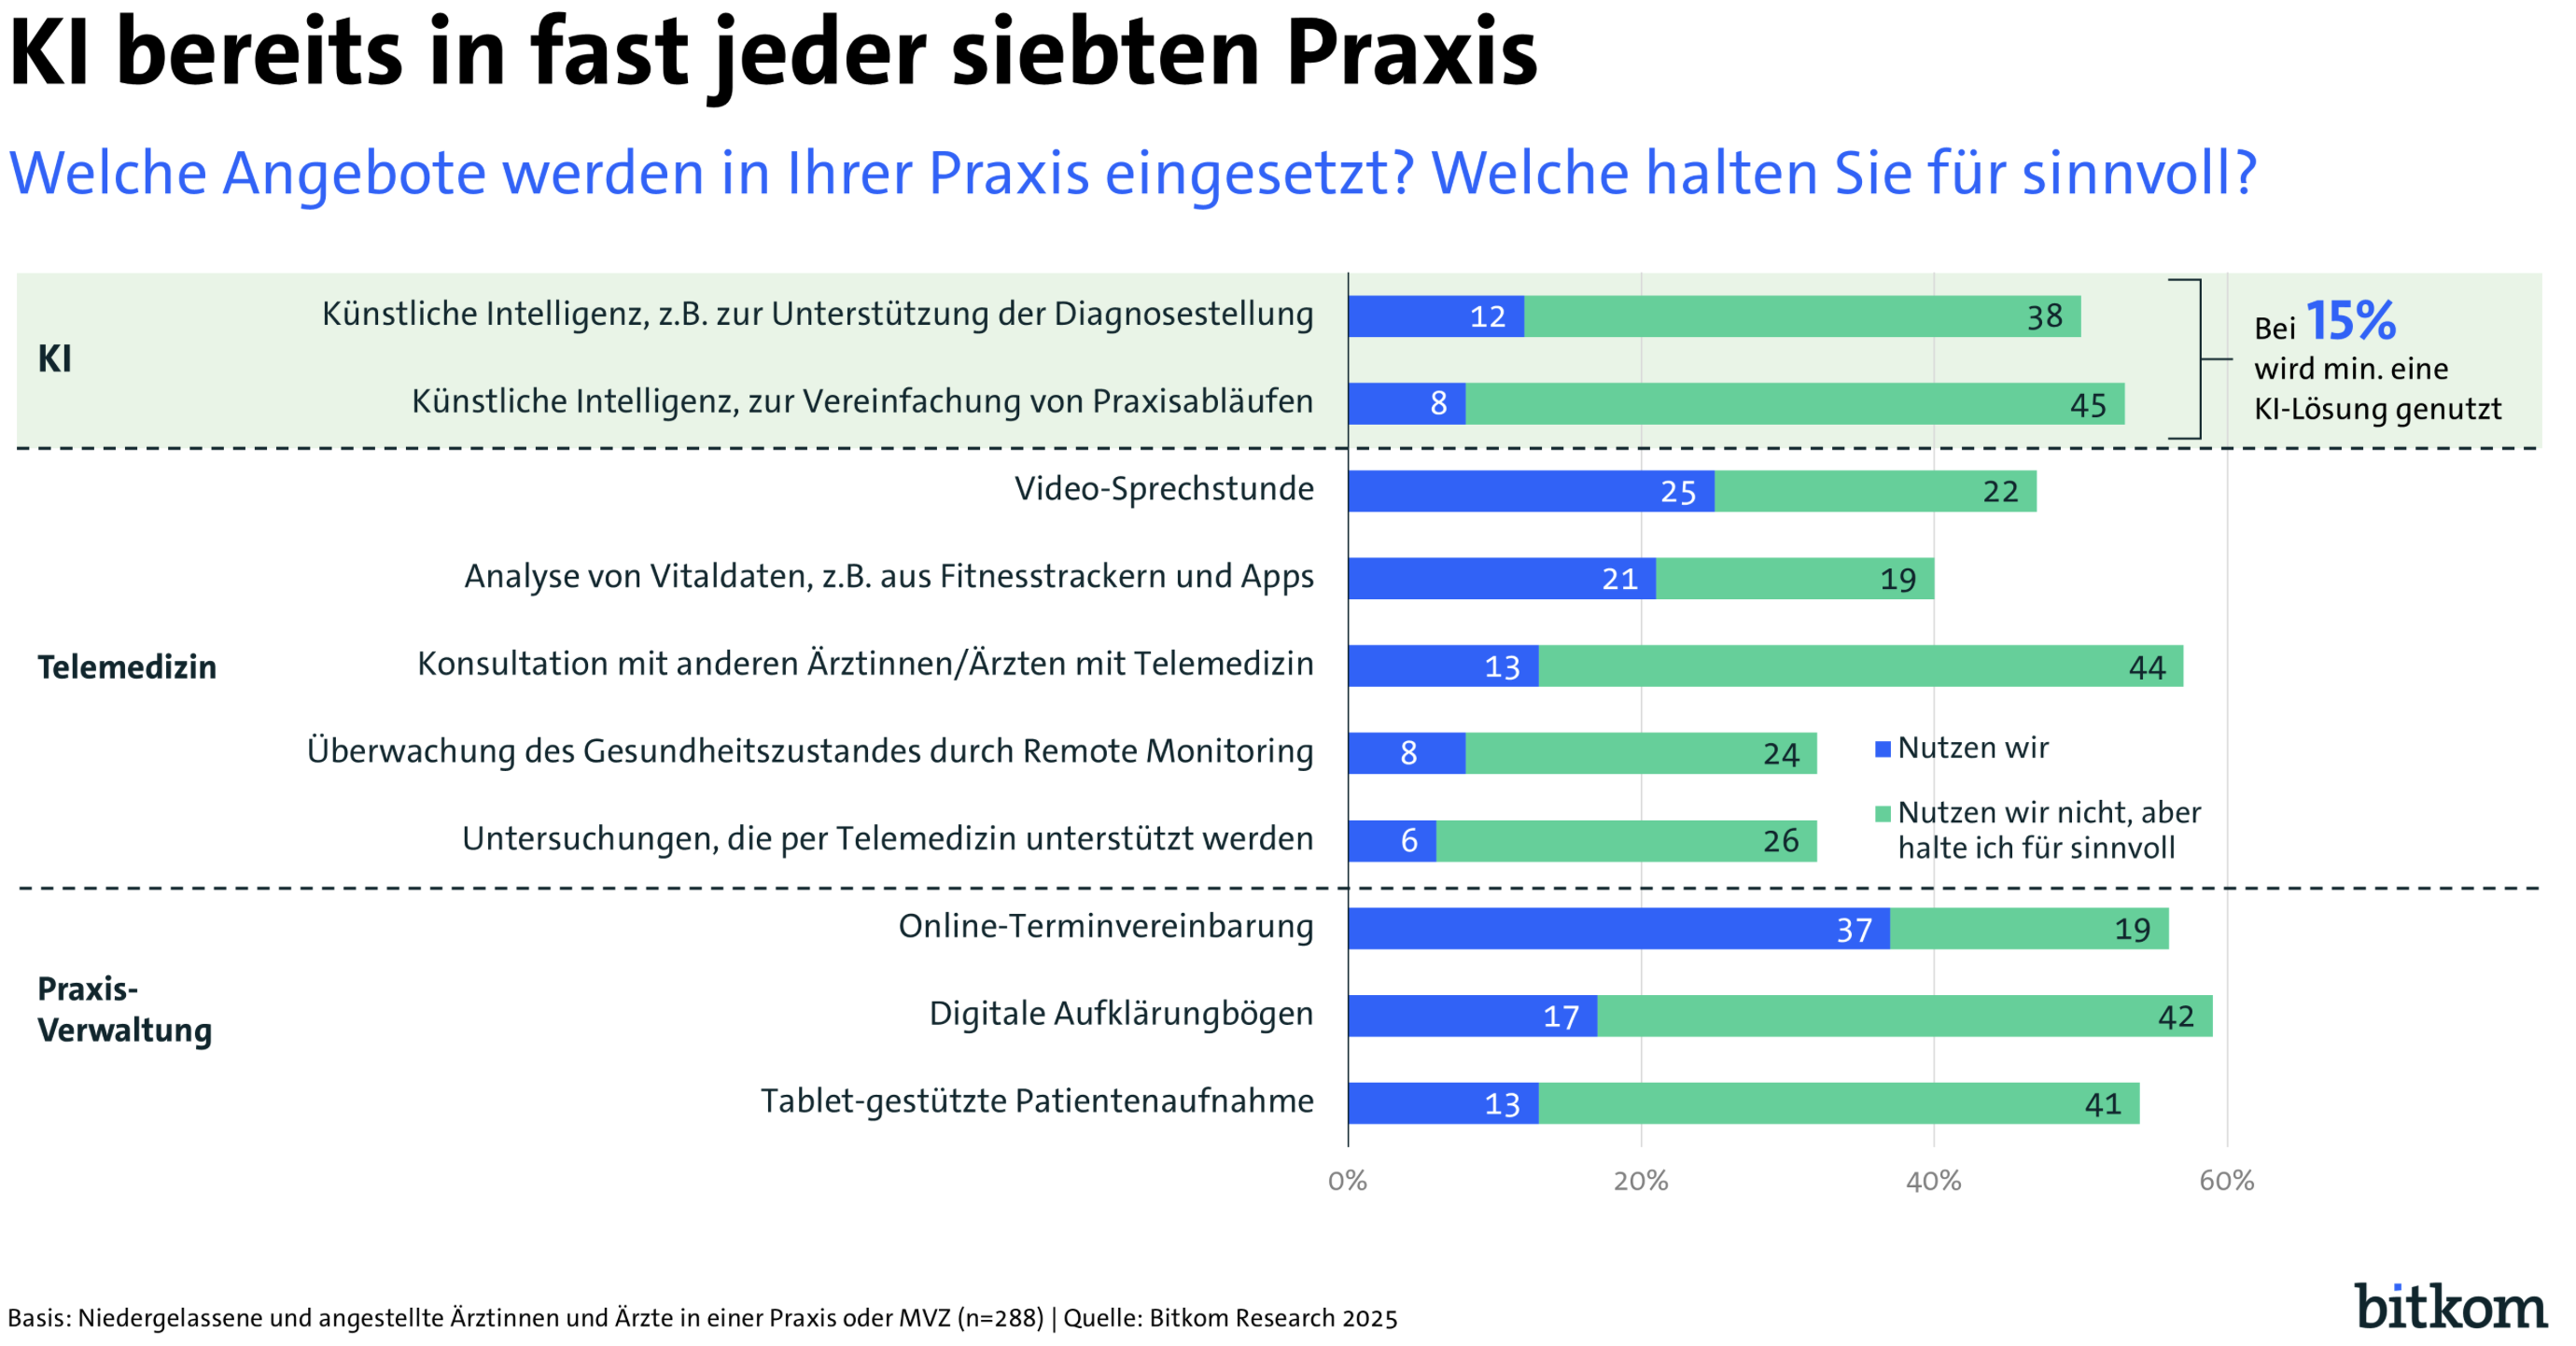
\includegraphics[width=3.5in]{Ki_nutzung}
	\caption{\cite{ref:bitkom2025} KI-Nutzung in Arztpraxen 2025 | Quelle: Bitkom Research, 2025}
	\label{fig:Ki_nutzung}
\end{figure}
	

\section{Wie funktioniert Künstliche Intelligenz}

Die Funktionsweise moderner Systeme der Künstlichen Intelligenz (KI) basiert im Kern auf der Fähigkeit, große Datenmengen zu verarbeiten und darin Muster sowie statistische Zusammenhänge zu erkennen. Ein zentrales Konzept hierbei sind künstliche neuronale Netze, die dem Aufbau biologischer Neuronen nachempfunden sind und Informationen in mehreren hierarchischen Schichten verarbeiten \cite{ref:alexander}.

Neuronale Netze bestehen aus einem Input-Layer, mehreren Hidden-Layers und einem Output-Layer\footnote{Der Output-Layer ist die letzte Schicht des Netzwerks und produziert die endgültige Vorhersage oder Entscheidung. Bei einer medizinischen Diagnose könnte der Output-Layer beispielsweise eine Wahrscheinlichkeit zwischen 0 und 1 ausgeben, die anzeigt, ob eine bestimmte Krankheit vorhanden ist oder nicht.}. Jede Schicht wandelt die Aktivierungen der vorherigen Schicht mithilfe gewichteter Verbindungen um, sodass unterschiedliche Muster repräsentiert werden können \cite{ref:alexander}. Während des Trainingsprozesses werden die Gewichte zwischen den Neuronen schrittweise angepasst, sodass das Netzwerk zunehmend aussagekräftige Merkmalsrepräsentationen lernt und schließlich in der Lage ist, Muster zu erkennen und zu generalisieren \cite{ref:alexander}.

Dieser Prozess hängt jedoch entscheidend von der Qualität der Trainingsdaten ab. Neuronale Netze lernen ausschließlich aus den Mustern in ihren Daten - sie können daher nur so zuverlässig sein wie die Daten, auf denen sie trainiert wurden\cite{ref:morhammed2025}. Diese Abhängigkeit von guter Datenqualität ist entscheidend, um die Zuverlässigkeit KI-gestützter Diagnosen zu verstehen und zeigt, warum strenge Validierungsverfahren notwendig sind.

	% ================= II. GRUNDLAGEN & CHANCEN ===============

\section{Chancen von KI in Wissenschaft und Medizin}
\label{sec:chancen}

Künstliche Intelligenz (KI) ist zu einem wichtigen Werkzeug in der biomedizinischen Forschung und Patientenversorgung geworden. Datengetriebene Verfahren des maschinellen Lernens und Deep Learning kommen inzwischen routinemäßig für Bildanalyse, Prognosemodelle und wissenschaftliche Auswertungen zum Einsatz\cite{ref:hai2025aiindex}. Diese Entwicklung wird durch die Verfügbarkeit großer Datenmengen, spezialisierter Hardware und leistungsfähiger Foundation Models vorangetrieben, die komplexe Muster in klinischen und biomedizinischen Daten erkennen können\cite{ref:hai2025aiindex}.

	
\subsection{Grundbegriffe und Anwendungsfelder}
\label{subsec:grundbegriffe}

\emph{Machine Learning} (ML) umfasst Modelle, die aus Beispieldaten statistische Zusammenhänge lernen, anstatt über explizite Regeln programmiert zu werden. Häufig handelt es sich um überwachte Lernverfahren, bei denen Eingabedaten mit bekannten Zielgrößen (z. B. Diagnoselabels oder Ereignissen wie Rehospitalisation) verknüpft werden. \emph{Deep Learning} (DL) bezeichnet ML-Methoden mit tiefen neuronalen Netzen und ist insbesondere für Bild-, Text- und Sequenzdaten relevant\cite{ref:hai2025aiindex}. Auch generative Modelle und große Sprachmodelle werden vermehrt eingesetzt, um natürliche Sprache und multimodale klinische Informationen zu verarbeiten. In der Medizin finden solche Modelle typischerweise Verwendung in klinischen Entscheidungsunterstützungssystemen, die Diagnosen, Risikoprognosen oder Therapieentscheidungen ergänzen\cite{ref:hai2025aiindex}.

Typische Anwendungsfelder sind:
\begin{itemize}
	\item \textbf{Bildgebende Diagnostik:} In Radiologie und Pathologie analysieren DL-Modelle Röntgen-, CT- und MRT-Daten oder histologische Schnitte, markieren auffällige Regionen und unterstützen bei der Befundung\cite{ref:hai2025aiindex}. Sie können z. B. unauffällige Fälle aussortieren oder Verdachtsbefunde priorisieren und so den Workflow strukturieren.
	\item \textbf{Klinische Prognose und Risikobewertung:} ML-Modelle verarbeiten tabellarische klinische Daten, Laborwerte oder Vitalparameter, um Komplikations- oder Rehospitalisierungsrisiken abzuschätzen\cite{ref:hai2025aiindex}. Solche Modelle werden zunehmend in Scoringsysteme integriert und können behandelnde Teams bei der Triage und Therapieplanung unterstützen.
	\item \textbf{Biomedizinische Forschung:} Modellfamilien für Proteinsequenzen und -strukturen sowie multimodale Modelle unterstützen die Identifikation neuer Zielstrukturen und Wirkstoffkandidaten\cite{ref:hai2025aiindex}. Dadurch werden hochdimensionale Omics-Daten und große Literaturkorpora systematischer nutzbar.
\end{itemize}

Im Fokus dieser Arbeit stehen datengetriebene KI-Systeme, die auf großen medizinischen oder biomedizinischen Datensätzen trainiert werden und in Diagnostik, Prognose und Forschung zum Einsatz kommen\cite{ref:hai2025aiindex}. Regelbasierte Expertensysteme und rein administrative Automatisierung werden dagegen nur am Rand berücksichtigt.

	
	
\subsection{Chancen und Nutzen}
\label{subsec:chancen_nutzen}

Die beschriebenen Systeme bieten vielfältige Potenziale für Wissenschaft und medizinische Praxis. Diese betreffen sowohl die Qualität klinischer Entscheidungen als auch Effizienzgewinne und neue Formen der Wissensgenerierung.

\paragraph{Steigerung der diagnostischen Qualität}

Aktuelle klinische Studien belegen, dass KI-Modelle in bestimmten diagnostischen Bildgebungsaufgaben vergleichbare oder bessere Leistungen als Expert:innen erzielen\cite{ref:hai2025aiindex}\cite{ref:faiyazuddin2025}. In einigen Szenarien ließen sich beispielsweise Sensitivität und Detektionsraten für frühe oder subtile Befunde erhöhen, während gleichzeitig die Bearbeitungszeit pro Untersuchung sank\cite{ref:faiyazuddin2025}. Besonders vielversprechend sind Human-AI-Teams, da sich deren Diagnosegenauigkeit in Studien teils als überlegen gegenüber Einzelentscheiden erwies\cite{ref:hai2025aiindex}. KI-Systeme können dabei als „zweite Lesung" fungieren, systematisch auf inkonsistente Befunde hinweisen und die interindividuelle Variabilität zwischen Befunder:innen reduzieren.

\paragraph{Präzisionsmedizin und neue wissenschaftliche Einsichten}

Große Modellarchitekturen für Proteinstrukturen und biologische Sequenzen erlauben es, komplexe Zusammenhänge in Omics-Daten besser zu erfassen und Strukturinformationen in bisher unerreichtem Umfang zu generieren\cite{ref:hai2025aiindex}. Dies ermöglicht neue Hypothesen in Biologie und Pharmakologie, beispielsweise bei der Suche nach geeigneten Wirkstoffbindestellen oder der Bewertung funktioneller Konsequenzen von Varianten. In der klinischen Forschung können ML-Modelle Patient:innen in Subgruppen mit unterschiedlichen Risikoprofilen einteilen und so personalisierte Therapieansätze oder stratifizierte Studiendesigns unterstützen.

\paragraph{Effizienzgewinne und Entlastung klinischer Teams}

Ökonomische Analysen zeigen, dass KI in vielen medizinischen Sektoren messbare Produktivitätsgewinne ermöglicht, insbesondere durch Automatisierung repetitiver Tätigkeiten wie Vorbefundung, Triage und Dokumentation\cite{ref:hai2025aiindex}\cite{ref:faiyazuddin2025}. In der Versorgungspraxis kann dies dazu beitragen, Befundungsstaus zu reduzieren und zeitkritische Fälle schneller zu bearbeiten. Synthetische Daten werden zudem als Option für datenschutzkonforme Trainingsdatensätze und das Abbilden seltener Szenarien diskutiert\cite{ref:hai2025aiindex}. Erste Evaluationsstudien zeigen jedoch, dass Effizienzgewinne nur dann realisiert werden, wenn KI-Systeme in bestehende klinische Workflows integriert und Aufgaben klar zwischen Mensch und System verteilt sind\cite{ref:faiyazuddin2025}.

\paragraph{Gesellschaftlicher Nutzen und Akzeptanz}

Befragungen zeigen, dass viele Menschen KI-Anwendungen als nützlich wahrnehmen und deren Einfluss auf Alltag und Gesundheit erwarten; jedoch besteht weiterhin Skepsis bezüglich ethischer Standards und der Realisierbarkeit versprochener Vorteile\cite{ref:hai2025aiindex}. Für das Gesundheitswesen bedeutet dies, dass neben technischen Leistungskennzahlen auch Aspekte wie Transparenz, Nachvollziehbarkeit und Beteiligung von Patient:innen eine Rolle für die Akzeptanz spielen. Realistisch kommunizierte Grenzen der Systeme und sorgfältig gestaltete Aufklärung können dazu beitragen, überzogene Erwartungen und unbegründete Ängste gleichermaßen zu vermeiden.

	% ================= III. RISIKEN, REPRODUZIERBARKEIT, BIAS ===============
	
\section{Risiken und wissenschaftliche Herausforderungen}
\label{sec:risiken}

Mit dem zunehmenden Einsatz von KI in sicherheitskritischen Kontexten steigen die Anforderungen an Qualität und Transparenz der zugrunde liegenden Studien. Klassische Leistungskennzahlen nähern sich inzwischen teils der Sättigung, während zentrale Fragen zu Robustheit, Fairness und langfristigem Verhalten vieler Systeme offen bleiben\cite{ref:hai2025aiindex}. Für eine fundierte Bewertung des Nutzens von KI in der Medizin müssen daher nicht nur technische Benchmarks, sondern auch methodische und ethische Kriterien der Studiengestaltung berücksichtigt werden.

\subsection{Reproduzierbarkeit von KI-Ergebnissen}
\label{subsec:reproduzierbarkeit}

Reproduzierbarkeit bedeutet, dass unabhängige Gruppen unter ähnlichen Bedingungen zu kongruenten Ergebnissen gelangen. Für medizinische KI umfasst das insbesondere:
\begin{itemize}
	\item transparente Beschreibung von Datensätzen und deren Vorverarbeitung,
	\item robuste Evaluationsprotokolle mit externer Validierung,
	\item nachvollziehbare Dokumentation der Modellarchitektur und Hyperparameter\cite{ref:hai2025aiindex}.
\end{itemize}

In der Praxis erfüllen viele Publikationen zu KI in der Medizin diese Anforderungen nur teilweise\cite{ref:hai2025aiindex}. Unzureichend dokumentierte Vorverarbeitungsschritte, intransparente Datensplits oder fehlende externe Validierung erschweren es, Ergebnisse nachzuvollziehen oder auf neue Populationen zu übertragen. Hinzu kommt, dass Modellverhalten stark von Randbedingungen wie Scannerhardware, Prävalenzen oder lokalen Behandlungspfaden abhängen kann. Für die Patient:innensicherheit ist daher entscheidend, dass Studien klare Informationen zu Kontext, Limitierungen und Generalisierbarkeit der Modelle liefern.



\subsection{Bias und Fairness}



\label{subsec:bias_fairness}


Bias tritt auf, wenn Vorhersagen systematisch bestimmte Gruppen benachteiligen, etwa aufgrund einseitiger Trainingsdaten oder ungeeigneter Zielgrößen\cite{ref:hai2025aiindex}\cite{ref:celi2022bias}. Das Vertrauen, dass KI diskriminierungsfrei agiert, ist laut Umfragen gesunken. Wissenschaftliche Studien fordern daher, Leistungsvergleiche in relevanten Subgruppen (Geschlecht, Alter, Ethnie) zu berichten und Zielgrößen kritisch zu wählen\cite{ref:celi2022bias}\cite{ref:hai2025aiindex}. Neben deskriptiven Analysen gewinnt auch die explizite Messung von Fairness an Bedeutung, etwa durch Metriken, die Fehlerraten oder Kalibrierung zwischen Gruppen vergleichen\cite{ref:celi2022bias}. 

Zur Reduktion von Bias werden Ansätze entlang der gesamten Entwicklungskette diskutiert: von der gezielten Diversifizierung und Dokumentation von Datensätzen über anpassbare Schwellenwerte in verschiedenen Subgruppen bis hin zu algorithmischen Korrekturverfahren\cite{ref:celi2022bias}\cite{ref:hai2025aiindex}. Für die Praxis bleibt jedoch zentral, dass potenzielle Verzerrungen offengelegt werden und klinische Entscheidungen nicht unkritisch automatisiert übernommen werden.

\subsection{Transparenz und Erklärbarkeit (Explainable AI)}
\label{subsec:xai}

Viele leistungsfähige Modelle verhalten sich für Nutzer:innen wie Black Boxes. Deshalb sind Transparenz auf Systemebene (Trainingsdaten, Modellgrenzen, Evaluationsprotokolle) und Erklärbarkeit auf Fallniveau (z. B. Heatmaps, Feature Attribution) entscheidend\cite{ref:hai2025aiindex}\cite{ref:chen2022}. Studien aus der medizinischen Bildgebung warnen jedoch davor, Erklärungen unkritisch als „Wahrheit" zu interpretieren: Saliency-Maps können beispielsweise scheinbar plausible Visualisierungen liefern, ohne dass diese tatsächlich kausal mit der Vorhersage verknüpft sind\cite{ref:chen2022}.

Aus human-zentrierter Perspektive ist daher weniger eine perfekte Erklärung als vielmehr eine sinnvolle Unterstützung der ärztlichen Entscheidungsfindung entscheidend\cite{ref:chen2022}. Dazu gehört, dass Unsicherheiten, Anwendungsgrenzen und typische Fehlermuster der Modelle klar kommuniziert werden und dass Nutzer:innen Werkzeuge erhalten, mit denen sie Vorhersagen hinterfragen können. Human-AI-Teams profitieren dann am meisten, wenn die Nutzer:innen die Stärken und Schwächen des Modells einschätzen können und Unterstützung nicht unreflektiert übernehmen.

Transparenz und Erklärbarkeit sind somit nicht nur ethische Anforderungen, sondern zentrale Bedingungen für eine sichere Integration in den Versorgungsalltag\cite{ref:hai2025aiindex}\cite{ref:chen2022}. Sie bilden zugleich eine wichtige Schnittstelle zu regulatorischen Vorgaben (z. B. Medizinprodukte-Regulierung) und zum Konzept des Human-AI-Teamings, das in den weiteren Kapiteln vertieft wird.

	
	
		\section{Valide Studien und Evaluationsprotokolle}

	
	Die Bewertung der Zuverlässigkeit KI-basierter medizinischer Systeme erfordert standardisierte und transparent dokumentierte Evaluationsprotokolle. Im Gegensatz zu klassischen Softwareprodukten entsteht die diagnostische Leistung einer KI nicht primär durch deterministische Algorithmen, sondern durch statistische Muster, die aus Trainingsdaten extrahiert wurden. Daher hängt die klinische Validität maßgeblich von der Qualität der Datenbasis, dem Studiendesign sowie der Robustheit der verwendeten Evaluationsmetriken ab. Zahlreiche aktuelle Leitlinien, darunter Empfehlungen der WHO sowie regulatorische Anforderungen der FDA und der EU, betonen die Notwendigkeit nachvollziehbarer und reproduzierbarer Verfahren zur Bewertung KI-basierter Diagnostik \cite{ref:whoai2021,ref:fdaprinciples,ref:ema2023ai}.
	
		\subsection{Datenbasis und Studiendesign}
	
	Ein zentraler Aspekt valider Evaluationsprotokolle ist eine repräsentative und qualitativ hochwertige Datenbasis. Für medizinische KI-Systeme bedeutet dies, dass die Datensätze ausreichend heterogen sein müssen, um verschiedene Kliniken, Aufnahmegeräte, Patientengruppen und Erkrankungsausprägungen abzudecken. Homogene Trainingsdaten führen häufig zu Modellen, die nur im ursprünglichen Kontext gut funktionieren, jedoch bei veränderten Bedingungen deutliche Leistungseinbußen zeigen \cite{ref:geirhos2020shortcut}. Derartige Domänenverschiebungen sind insbesondere in der medizinischen Diagnostik kritisch, da Fehlklassifikationen direkte Auswirkungen auf Patientensicherheit haben.
	
	Best Practices empfehlen eine klare Trennung der Daten in Trainings-, Validierungs- und Testmengen sowie den Einsatz einer externen Validierung, bei der das Modell auf unabhängigen Datensätzen evaluiert wird \cite{ref:kohane2019key}. Externe Validierung gilt als Goldstandard, da sie den Einsatz in realen klinischen Umgebungen realistischer abbildet. Studien zeigen, dass Modelle ohne externe Validierung häufig systematisch zu positiv bewertet werden und im klinischen Alltag schlechter abschneiden \cite{ref:liu2019comparison}. Darüber hinaus sollten alle Schritte der Datenaufbereitung - etwa Normalisierung, Segmentierung oder Annotierungsprozesse - detailliert dokumentiert werden, um Selektions- oder Messbias zu vermeiden.
	
	\subsection{Evaluationsmetriken f\"ur diagnostische KI}

	Zur Bewertung diagnostischer Leistung werden etablierte Metriken aus der medizinischen Statistik eingesetzt. Die wichtigsten Kennzahlen umfassen Sensitivität (True-Positive-Rate), Spezifität (True-Negative-Rate), Genauigkeit sowie der F1-Score \cite{ref:jurman2012comparison}. Bei ungleich verteilten Klassen - beispielsweise seltenen Erkrankungen – ist die Genauigkeit jedoch wenig aussagekräftig. In diesen Fällen sind Metriken wie die AUC-ROC (Area Under the Receiver Operating Characteristic Curve) oder die Precision-Recall-AUC besser geeignet, da sie die Modellleistung bei unausgeglichenen Klassen realistischer abbilden \cite{ref:saito2015precision}.
	
	Für klinische Bewertungen spielt zudem die sogenannte „Clinical Utility“ eine Rolle. Diese berücksichtigt, wie sich ein falsch-positiver oder falsch-negativer Befund auf klinische Entscheidungen auswirkt. Moderne Studien kombinieren daher statistische Leistungsmaße mit klinischen Endpunkten, etwa veränderten Therapieentscheidungen oder Diagnosezeiten \cite{ref:brat2020realworld}. Nur durch diesen integrativen Ansatz lässt sich ermitteln, ob eine KI nicht nur statistisch gut performt, sondern auch klinisch sinnvoll eingesetzt werden kann.
	
	\subsection{Vergleich mit Expert:innen und klinische Studien}

	Ein häufig genutzter Ansatz zur Bewertung diagnostischer KI-Systeme ist der direkte Vergleich mit Ärztinnen und Ärzten. In sogenannten Reader-Studies analysieren mehrere medizinische Fachpersonen denselben Datensatz, sodass die Leistung der KI mit menschlicher Expertise verglichen werden kann \cite{ref:lakhani2017deep}. Multireader-Multicase-Studien (MRMC) gelten als besonders robust, da sie sowohl interindividuelle Unterschiede zwischen Expert:innen als auch fallabhängige Schwankungen berücksichtigen \cite{ref:berbaum1992mrmc}. Diese Studienform ermöglicht es, objektiv zu beurteilen, ob ein KI-Modell diagnostisch mindestens gleichwertig oder besser als klinisches Fachpersonal arbeitet.
	
	Für den Einsatz im medizinischen Alltag reicht eine Reader-Study jedoch nicht aus. Regulatorische Richtlinien wie die MDR oder FDA-Leitlinien fordern prospektive Studien im realen klinischen Workflow \cite{ref:fdaprinciples}. Solche Studien evaluieren, wie sich die KI auf tatsächliche Entscheidungen auswirkt, ob Ärztinnen und Ärzte die Modelle korrekt interpretieren und wie zuverlässig die Systeme unter variierenden Bedingungen funktionieren. Prospektive Studien gelten daher als höchste Evidenzstufe, sind jedoch organisatorisch und ethisch anspruchsvoll.
	
	\subsection{Dokumentation und Reproduzierbarkeit}

	Ein wesentlicher Grundsatz wissenschaftlicher Arbeit ist die Reproduzierbarkeit. Viele KI-Studien scheitern jedoch daran, dass zentrale Informationen zur Datenvorbereitung, Modellarchitektur oder Hyperparameterwahl unzureichend dokumentiert sind. Dies führt zu einem Reproduzierbarkeitsproblem, das die Glaubwürdigkeit wissenschaftlicher Ergebnisse untergräbt \cite{ref:hutson2018reproducibility}. Aus diesem Grund fordern internationale Organisationen umfangreiche Dokumentationsstandards, wie etwa die WHO-Guidelines zur KI in der Medizin oder das CONSORT-AI-Framework \cite{ref:consortai2020}.
	
	Empfohlen wird eine vollständige Offenlegung aller verwendeten Datenquellen, Vorverarbeitungsschritte, Modellversionen, Hyperparameter und Softwarebibliotheken. Darüber hinaus sollten Modelle versioniert und - sofern rechtlich möglich - öffentlich zugänglich gemacht werden. Nur durch transparente Dokumentation lässt sich sicherstellen, dass andere Forschungsgruppen die Ergebnisse unabhängig prüfen und validieren können.
	
	% ================= V. REGULATORIK & ETHIK =====================
	\section{Regulatorische und ethische Rahmenbedingungen}

	Neben der wissenschaftlichen Validität spielen regulatorische und ethische Aspekte eine zentrale Rolle beim Einsatz KI-basierter Diagnosesysteme. Da Fehlentscheidungen direkte gesundheitliche Risiken bergen, unterliegen KI-Systeme in der Medizin strengen Anforderungen hinsichtlich Sicherheit, Transparenz und Datenverarbeitung.
	
	\subsection{KI als Medizinprodukt und die EU-MDR}

	Die europäische Medizinprodukteverordnung (MDR) definiert klare Kriterien zur Einstufung von Software als Medizinprodukt. Diagnostische KI-Systeme fallen in der Regel unter die Risikoklasse IIa oder höher, wodurch hohe Anforderungen an klinische Evidenz, Risikobewertungen und technische Dokumentation entstehen \cite{ref:mdr2017}. Hersteller müssen nachweisen, dass das Modell robust, sicher und klinisch validiert ist und keine systematischen Diskriminierungen verursacht. Darüber hinaus verlangt die MDR eine kontinuierliche Überwachung nach der Markteinführung („Post-Market Surveillance“), um Leistungsabfälle, Bias-Effekte oder Fehlfunktionen frühzeitig zu erkennen \cite{ref:ema2023ai}.
	
	\subsection{Datenschutz und ethische Aspekte}

	Die Verarbeitung medizinischer Daten unterliegt strengen datenschutzrechtlichen Vorgaben der DSGVO. Besonders relevant sind Anforderungen an Datensparsamkeit, Zweckbindung und die informierte Einwilligung der Patientinnen und Patienten \cite{ref:dsgvo2018}. Für KI-Systeme stellt dies eine Herausforderung dar, da Modelle häufig große, vielfältige und langfristig genutzte Datensätze benötigen. Zudem entstehen ethische Fragen hinsichtlich Fairness, Verantwortlichkeit und Transparenz. Fehlentscheidungen müssen nachvollziehbar sein, und es muss klar geregelt werden, wer im Fehlerfall haftet - der Hersteller, die behandelnde Person oder die Einrichtung \cite{ref:floridi2022ethics}. Internationale Leitlinien betonen daher die Notwendigkeit eines verantwortungsvollen Human-AI-Teaming, in dem KI als Unterstützung, nicht aber als alleiniger Entscheider fungiert \cite{ref:whoai2021}.
	
	
	
	% ================= VI. HUMAN-AI-TEAMING ========================
	\section{Human-AI-Teaming in der medizinischen Praxis}
	% Ziel: deutlich machen, dass KI nicht alles allein entscheiden soll.
	\label{sec:human_ai_teaming}
	
	Die zuvor beschriebenen Chancen und Risiken machen deutlich, dass KI-Systeme in der Medizin nicht als autonome Entscheidungsträger verstanden werden sollten, sondern als Werkzeuge, die menschliche Expertise ergänzen. Anstatt Ärztinnen und Ärzte zu ersetzen, zielt \emph{Human-AI-Teaming} darauf ab, Stärken von Mensch und Maschine sinnvoll zu kombinieren: KI übernimmt wiederkehrende, datenintensive Aufgaben, während klinische Verantwortung, Kontextbewertung und ethische Abwägungen beim Menschen verbleiben\cite{ref:hai2025aiindex}\cite{ref:faiyazuddin2025}.
	
	
	\subsection{Rollenverteilung zwischen Mensch und KI}

	\label{subsec:rollenverteilung}
	
	Eine zentrale Voraussetzung für sicheres Human-AI-Teaming ist eine klare Rollenverteilung. In der Praxis lassen sich grob drei Rollenbilder unterscheiden:
	
	\begin{itemize}
		\item \textbf{KI als Screening- oder Triage-System:} In bildgebenden Fächern kann KI zunächst unkritische Fälle identifizieren, auffällige Befunde priorisieren und so Worklists sortieren. Die endgültige Befundung bleibt bei der Radiologin bzw. dem Radiologen, der KI-Vorschläge prüfen und ggf. korrigieren kann\cite{ref:hai2025aiindex}.
		\item \textbf{KI als Zweitmeinung:} In komplexen oder unsicheren Fällen kann ein Modell eine alternative Einschätzung liefern, etwa einen zusätzlichen Risikoscore oder eine differenzialdiagnostische Rangliste. Solche Systeme werden häufig mit einem „override“-Prinzip implementiert, bei dem Menschen Entscheidungen jederzeit verwerfen können\cite{ref:faiyazuddin2025}.
		\item \textbf{KI als Workflow-Assistenz:} Große Sprachmodelle und andere KI-Werkzeuge unterstützen bei Dokumentation, Strukturierung von Anamnesen, Inbox-Nachrichten oder der Extraktion relevanter Informationen aus Krankenakten\cite{ref:Artsi.2025}. Die ärztliche Entscheidung selbst wird dadurch vorbereitet, aber nicht automatisiert getroffen.
	\end{itemize}
	
	Studien deuten darauf hin, dass Human-AI-Teams in einigen Szenarien bessere Leistungen erzielen als Mensch oder KI allein, etwa durch höhere Sensitivität bei gleichzeitig kontrollierter Spezifität\cite{ref:hai2025aiindex}\cite{ref:faiyazuddin2025}. Voraussetzung ist jedoch, dass die Verantwortlichkeiten eindeutig geregelt sind: Klinische Entscheidungen und die Aufklärung der Patient:innen liegen rechtlich weiterhin beim medizinischen Personal; KI-Ausgaben haben den Charakter von Empfehlungen und müssen in den individuellen Kontext eingeordnet werden.
	
	Darüber hinaus erfordert Human-AI-Teaming organisatorische Regeln: Wer darf ein System nutzen? In welchen Situationen ist eine KI-Empfehlung verpflichtend einzuholen (z. B. bei Triage)? Wie werden widersprüchliche Bewertungen zwischen Mensch und System dokumentiert und aufgelöst? Solche Fragen sind eng mit regulatorischen Rahmenbedingungen (z. B. MDR) und internen klinischen Leitlinien verknüpft.
	
	\subsection{Vertrauen, Akzeptanz und Usability}

	
	\label{subsec:vertrauen}
	
	Ob Human-AI-Teams in der Praxis funktionieren, hängt wesentlich von Vertrauen, Akzeptanz und der Gebrauchstauglichkeit (Usability) der Systeme ab. Untersuchungen zeigen, dass Fachpersonal zwar grundsätzlich offen für KI-Unterstützung ist, aber Vorbehalte gegenüber Intransparenz, potenziellen Biases und ungeklärter Haftung hat\cite{ref:hai2025aiindex}\cite{ref:celi2022bias}\cite{ref:faiyazuddin2025}. Auch Patient:innen bringen ambivalente Erwartungen mit: Viele sehen Chancen für bessere Diagnostik, befürchten aber gleichzeitig Verlust persönlicher Zuwendung und unfaire Entscheidungen\cite{ref:hai2025aiindex}.
	
	Aus Sicht der Mensch-Maschine-Interaktion lassen sich mehrere Faktoren für Vertrauen und Akzeptanz identifizieren\cite{ref:chen2022}\cite{ref:Artsi.2025}:
	
	\begin{itemize}
		\item \textbf{Transparenz und Erklärbarkeit:} Nutzer:innen müssen verstehen können, welche Daten ein Modell verwendet, welche Unsicherheiten bestehen und wo seine Grenzen liegen. Erklärungen sollten dabei nicht nur „technisch korrekt“, sondern für die Zielgruppe verständlich und arbeitsplatznah gestaltet sein.
		\item \textbf{Gutes User Interface und Workflow-Integration:} KI-Ausgaben müssen zur richtigen Zeit am richtigen Ort erscheinen, etwa direkt im Befundungssystem oder in der elektronischen Patientenakte, anstatt in separaten Portalen. Umständliche Bedienung oder Medienbrüche reduzieren Akzeptanz, auch wenn die Modellleistung gut ist\cite{ref:Artsi.2025}.
		\item \textbf{Kalibrierte Zuverlässigkeit:} Für das Vertrauen ist weniger die maximal erreichbare Genauigkeit entscheidend als ein gut kalibriertes Verhalten: Modelle sollten ihre Unsicherheit kommunizieren (z. B. durch Konfidenzangaben oder Warnhinweise), statt scheinbar sichere, aber potenziell falsche Ausgaben zu liefern.
		\item \textbf{Schulung und klare Verantwortlichkeiten:} Ärztliches und pflegerisches Personal muss nicht nur die Bedienung, sondern auch typische Fehlermuster der Systeme kennen. Schulungsprogramme, Standardarbeitsanweisungen(Standard Operating Procedures) und Leitlinien sollten festhalten, wie KI-Empfehlungen dokumentiert, hinterfragt und ggf. korrigiert werden\cite{ref:faiyazuddin2025}.
	\end{itemize}
	
	Human-zentrierte Designansätze betonen, dass Transparenz und Erklärbarkeit nicht allein Eigenschaften des Algorithmus sind, sondern aus der Interaktion von System, Nutzer:in und Kontext entstehen\cite{ref:chen2022}. Systematische Reviews zu erklärbarer medizinischer KI zeigen, dass viele bestehende Arbeiten zwar visuelle Erklärungen (z. B. Heatmaps) erzeugen, aber selten empirisch prüfen, ob diese Erklärungen Ärzt:innen tatsächlich bei Entscheidungen helfen\cite{ref:chen2022}. Hier besteht noch erheblicher Forschungsbedarf, insbesondere im Hinblick auf unterschiedliche Erfahrungsniveaus und Fachrichtungen.
	
	Aktuelle Übersichten zur Implementierung großer Sprachmodelle in klinischen Workflows berichten, dass frühe Anwendungen zwar häufig Effizienzgewinne und positive Nutzerfeedbacks zeigen, die Einführung aber durch regulatorische Unsicherheit, fehlende Monitoring-Konzepte und heterogene lokale Infrastrukturen erschwert wird\cite{ref:Artsi.2025}. Für robuste Human-AI-Teams sind daher nicht nur performante Modelle, sondern auch geeignete Governance-Strukturen, Monitoring und kontinuierliche Evaluation nötig.
	
	Insgesamt lässt sich festhalten, dass Human-AI-Teaming ein zentrales Bindeglied zwischen technischen Möglichkeiten und sicherer Versorgung darstellt. Rollenverteilung, Vertrauen, Akzeptanz und Usability sind dabei nicht nur „weiche“ Faktoren, sondern bestimmen maßgeblich, ob die in den vorangegangenen Kapiteln beschriebenen Chancen von KI in der Medizin tatsächlich in der Versorgungspraxis ankommen.
	
	
\section{Fazit und Ausblick}
%jungs sicherstellen dass wir die Forschungsfrage beantwortet haben!
Die vorliegende Arbeit zeigt, dass KI in Wissenschaft und Medizin ein erhebliches Potenzial zur Verbesserung diagnostischer Genauigkeit, zur Entlastung klinischer Teams und zur Beschleunigung biomedizinischer Forschung bietet. Gleichzeitig wird deutlich, dass zuverlässige und faire KI-Systeme eine belastbare Datenbasis, transparente Studienprotokolle sowie reproduzierbare und klinisch aussagekräftige Evaluationsverfahren benötigen. Insbesondere Aspekte wie Bias, Generalisierbarkeit und Erklärbarkeit bleiben zentrale Herausforderungen, die in zukünftigen Forschungs- und Entwicklungsprozessen stärker berücksichtigt werden müssen.

Regulatorische Vorgaben wie die europäische MDR und datenschutzrechtliche Rahmenbedingungen bilden einen wichtigen Ordnungsrahmen, der Sicherheit und Qualität gewährleisten soll. Für eine erfolgreiche Integration in den klinischen Alltag ist jedoch ebenso entscheidend, dass KI-Systeme in Human-AI-Teams eingebettet werden, in denen die Expertise der Fachkräfte mit den algorithmischen Stärken kombiniert wird.

Ausblickend besteht weiterer Forschungsbedarf bei der Entwicklung standardisierter Evaluationsprotokolle, beim Monitoring von KI-Systemen im realen Betrieb sowie bei Methoden zur Erhöhung von Transparenz und Fairness. Zukünftige KI-Modelle werden voraussichtlich stärker multimodal, erklärbarer und adaptiver sein. Damit diese Technologien jedoch verantwortungsvoll eingesetzt werden können, müssen wissenschaftliche Evidenz, technische Robustheit und ethische Prinzipien gleichermaßen berücksichtigt werden.

	% ===================== REFERENCES ==============================

	\begin{thebibliography}{99}
		
		
% QUELLEN NICHT LÖSCHEN!!!!


%Faiks Quellen
\bibitem{ref:epai}
Europäisches Parlament, ``Was ist künstliche Intelligenz und wie wird sie genutzt?'' Generaldirektion Kommunikation, 2023. [Online]. Verfügbar unter: \url{https://www.europarl.europa.eu/news/de/headlines/priorities/kunstliche-intelligenz-in-der-eu/20230601STO93804/ki-gesetz-erste-regulierung-der-kunstlichen-intelligenz}(letzter Zugriff: 05.11.2025).
		
\bibitem{ref:baekki}
Bundesärztekammer, ``Von ärztlicher Kunst mit Künstlicher Intelligenz: Künstliche Intelligenz in der Medizin,'' Positionspapier, 2025. [Online]. Available: \url{https://www.bundesaerztekammer.de/themen/aerzte/digitalisierung/ki-in-der-medizin}letzter Zugriff: 05.11.2025).

\bibitem{ref:bitkom2025}
Bitkom e.V. und Hartmannbund, 
„KI in fast jeder siebten Praxis und vielen Kliniken im Einsatz,“ 
Presseinformation, 27. Mai 2025. [Online].  
Verfügbar unter: \url{https://www.bitkom.org/Presse/Presseinformation/KI-in-Praxis-und-Kliniken-im-Einsatz}  
(Zugriff am: 10. Nov. 2025).

\bibitem{ref:alexander}
Grüning, Alexander, *Künstliche Neuronale Netze – Grundlagen und Entwicklungen; 
Künstliche Intelligenz; Einführung in die Künstliche Intelligenz*, 
Vorlesungspräsentationen, DHBW, unveröffentlichtes Lehrmaterial, 2025.



%Abschnitt von dieser Quellewurde weggelassen??
\bibitem{ref:kiundwir}
F. Schmiedchen, M. Hafner, A. von Gernler und K. P. Kratzer (Hrsg.), 
\textit{Künstliche Intelligenz und Wir: Stand, Nutzung und Herausforderungen der KI}. 
Springer Vieweg, Berlin, 2026. 
[Online]. Verfügbar unter: \url{https://doi.org/10.1007/978-3-662-71567-3} 
(letzter Zugriff: 17.11.2025).

\bibitem{ref:morhammed2025}
S. Morhammed, L. Budach, M. Feuerpfeil, N. Ihde, A. Nathansen, N. Noack, H. Patzlaff, F. Naumann und H. Harmouch, 
``The effects of data quality on machine learning performance on tabular data,'' 
\textit{Information Systems}, vol. 132, 2025, Art. Nr. 102549, ISSN 0306-4379. 
[Online]. Verfügbar unter: \url{https://www.sciencedirect.com/science/article/pii/S0306437925000341} 
(letzter Zugriff: 05.11.2025).  


\bibitem{ref:3b1b}
Grant Sanderson, ``Gradient descent, how neural networks learn,'' 3Blue1Brown, 2017.  
[Online]. Verfügbar unter: \url{https://www.3blue1brown.com/topics/neural-networks}  
(letzter Zugriff: 16.11.2025).


%nico Quellen
\bibitem{ref:hai2025aiindex}
Stanford Institute for Human-Centered Artificial Intelligence (HAI), 
\textit{Artificial Intelligence Index Report 2025}. 
Stanford University, 2025. [Online]. 
Verfügbar unter: \url{https://aiindex.stanford.edu} 
(letzter Zugriff: 05.11.2025).

\bibitem{ref:celi2022bias}
Celi, L. A., Cellini, J., Charpignon, M.-L., Dee, E. C., Dernoncourt, F., 
Eber, R., Mitchell, W. G., Moukheiber, L., Schirmer, J., Situ, J., 
Paguio, J., Park, J., Wawira, J. G., Yao, S., \& for MIT Critical Data, 
„Sources of bias in artificial intelligence that perpetuate health disparities,“ 
\textit{PLOS Digital Health}, 2022. [Online]. 
Verfügbar unter: \url{https://journals.plos.org/digitalhealth/article?id=10.1371/journal.pdig.0000022} 
(letzter Zugriff: 05.11.2025).

\bibitem{ref:faiyazuddin2025}
Faiyazuddin, M., Rahman, S. J. Q., Anand, G., Siddiqui, R. K., Mehta, R., 
Khatib, M. N., Gaidhane, S., Zahiruddin, Q. S., Hussain, A., \& Sah, R., 
„The Impact of Artificial Intelligence on Healthcare,“ 
\textit{National Library of Medicine}, 2025. [Online]. 
Verfügbar unter: \url{https://pmc.ncbi.nlm.nih.gov/articles/PMC11702416/} 
(letzter Zugriff: 05.11.2025).

\bibitem{ref:chen2022}
Chen, H., Gomez, C., Huang, C.-M., \& Unberath, M., 
„Explainable medical imaging AI needs human-centered design,“ 
\textit{Nature}, 2022. [Online]. 
Verfügbar unter: \url{https://www.nature.com/articles/s41746-022-00699-2} 
(letzter Zugriff: 05.11.2025).

\bibitem{ref:Artsi.2025}
Y. Artsi, V. Sorin, B. S. Glicksberg, P. Korfiatis, G. N. Nadkarni und E. Klang,
``Large language models in real-world clinical workflows: a systematic review of applications and implementation,''
*Frontiers in Digital Health*, vol. 7, 2025.  
[Online]. Verfügbar unter: \url{https://doi.org/10.3389/fdgth.2025.1659134} (letzter Zugriff: 25.11.2025).

%Nicolaj Quellen
\bibitem{ref:whoai2021}
World Health Organization,
``Ethics and Governance of Artificial Intelligence for Health,''
WHO, 2021.
[Online]. Available: https://www.who.int/publications/i/item/9789240029200

\bibitem{ref:fdaprinciples}
U.S. Food and Drug Administration,
``Proposed Regulatory Framework for Modifications to Artificial Intelligence/Machine Learning-Based Software as a Medical Device,''
FDA Discussion Paper, 2019.
[Online]. Available: https://www.fda.gov/media/122535/download

\bibitem{ref:ema2023ai}
European Medicines Agency,
``Reflection Paper on the Use of Artificial Intelligence (AI) in the Medicinal Product Lifecycle,''
EMA/819319/2021, 2023.
[Online]. Available: \url{https://www.ema.europa.eu/en/documents/scientific-guideline/reflection-paper-use-artificial-intelligence-ai-medicinal-product-lifecycle_en.pdf}

\bibitem{ref:geirhos2020shortcut}
R. Geirhos et al.,
``Shortcut Learning in Deep Neural Networks,''
\textit{Nature Machine Intelligence}, vol. 2, pp. 665–673, 2020.
doi: 10.1038/s42256-020-00257-z
[Online]. Available: \url{https://www.nature.com/articles/s42256-020-00257-z}

\bibitem{ref:kohane2019key}
Isaac S. Kohane,
``Framing the challenges of artificial intelligence in medicine,''
\textit{BMJ Quality \& Safety}, vol. 28, no. 7, 2019.
doi: 10.1136/bmjqs-2018-008551

\bibitem{ref:liu2019comparison}
X. Liu et al.,
``A Comparison of Deep Learning Performance Against Health-Care Professionals: A Systematic Review and Meta-Analysis,''
\textit{The Lancet Digital Health}, vol. 1, no. 6, 2019.
doi: 10.1016/S2589-7500(19)30123-2

\bibitem{ref:jurman2012comparison}
G. Jurman, R. Riccadonna, C. Furlanello,
``A Comparison of MCC and CEN Error Measures in Multi-Class Prediction,''
\textit{PLoS ONE}, vol. 7, no. 8, 2012.
doi: 10.1371/journal.pone.0041882

\bibitem{ref:saito2015precision}
T. Saito and M. Rehmsmeier,
``The Precision-Recall Plot Is More Informative than the ROC Plot When Evaluating Binary Classifiers on Imbalanced Datasets,''
\textit{PLOS ONE}, vol. 10, no. 3, 2015.
doi: 10.1371/journal.pone.0118432

\bibitem{ref:brat2020realworld}
Gabriel A Brat et al.,
``International electronic health record-derived COVID-19 clinical course profiles: the 4CE consortium,''
\textit{NPJ Digital Medicine}, vol. 3, 2020.
doi: 10.1038/s41746-020-0306-0

\bibitem{ref:lakhani2017deep}
P. Lakhani and B. Sundaram,
``Deep Learning at Chest Radiography: Automated Classification of Pulmonary Tuberculosis by Using Convolutional Neural Networks,''
\textit{Radiology}, vol. 284, no. 2, 2017.
doi: 10.1148/radiol.2017162326

\bibitem{ref:berbaum1992mrmc}
K. S. Berbaum,
``Evaluation of a digital workstation for interpreting neonatal examinations. A receiver operating characteristic study,''
\textit{Investigative Radiology}, vol. 27, no. 9, 1992.
doi: 10.1097/00004424-199209000-00016

\bibitem{ref:hutson2018reproducibility}
M. Hutson,
``Artificial Intelligence Faces Reproducibility Crisis,''
\textit{Science}, vol. 359, no. 6377, 2018.
doi: 10.1126/science.359.6377.725

\bibitem{ref:consortai2020}
L. Liu et al.,
``CONSORT-AI and SPIRIT-AI: New Reporting Guidelines for Clinical Trials Involving Artificial Intelligence,''
\textit{The Lancet Digital Health}, vol. 2, no. 10, 2020.
doi: 10.1016/S2589-7500(20)30218-1

\bibitem{ref:mdr2017}
European Union,
``Regulation (EU) 2017/745 on Medical Devices (MDR),''
Official Journal of the European Union, 2017.
[Online]. Available: https://eur-lex.europa.eu/legal-content/EN/TXT/?uri=CELEX:32017R0745

\bibitem{ref:dsgvo2018}
European Union,
``General Data Protection Regulation (GDPR),'' Regulation (EU) 2016/679, 2018.
[Online]. Available: https://eur-lex.europa.eu/eli/reg/2016/679/oj

\bibitem{ref:floridi2022ethics}
L. Floridi and J. Cowls,
``A Unified Framework of Five Principles for AI in Society,''
\textit{Harvard Data Science Review}, 2022.
doi: 10.1162/99608f92.8cd550d1

				
	\end{thebibliography}
	

	
\end{document}
